\section{Motor Set Up}
\resetassemblysteps

\assemblystep{Update the Firmware}
To prepare the motors for programming, open REV Hardware Client 2 and
connect the motor via USB-C. You will more than likely see the device
appear labeled ``Outdated REV Device'' under the hardware tab.

\begin{figure}[H]
\centering
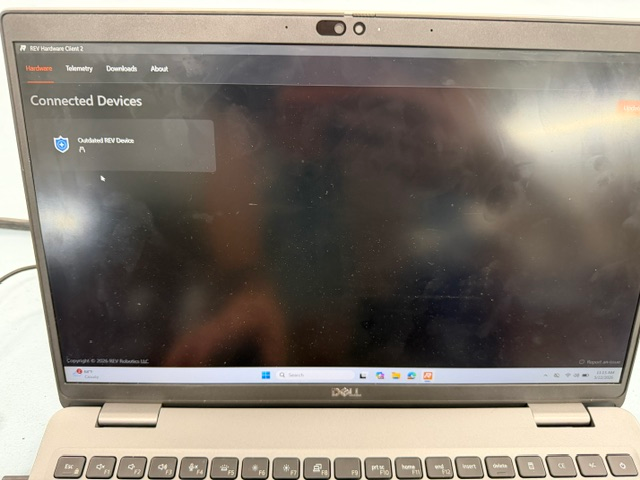
\includegraphics[width=0.5\textwidth]{media/image26.png}
\caption{An ``Outdated REV Device'' listed under the hardware tab.}
\end{figure}

Click on the device and instructions will appear to update the firmware.
Unplug the motor, use a thin object (like a small screwdriver) to press
and hold the Mode button on the motor, and reconnect to the computer.
Then release the Mode button.

\begin{figure}[H]
\centering
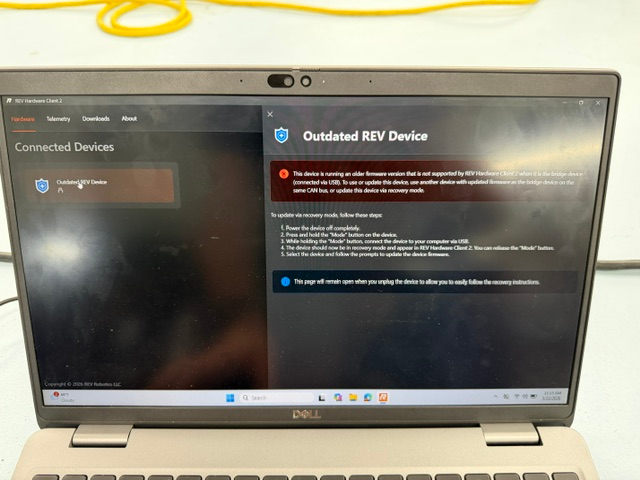
\includegraphics[width=0.47\textwidth]{media/image27.png}
\hfill
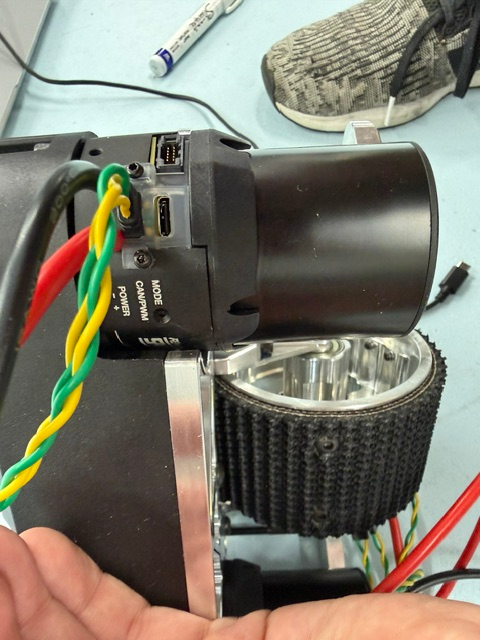
\includegraphics[width=0.47\textwidth]{media/image28.png}
\caption{Holding the Mode button with a thin tool while reconnecting the
motor over USB-C.}
\end{figure}

You will now see the motor label has changed to ``Recovery Device''.
Select SPARK Flex as device type and the latest firmware option and
click Install. After the install, be sure to click on the device, then Configuration, then the 3 dots at the bottom right, then factory reset. Failing to do so may result in the CAN ID being reset after a low battery shutdown.

\begin{figure}[H]
\centering
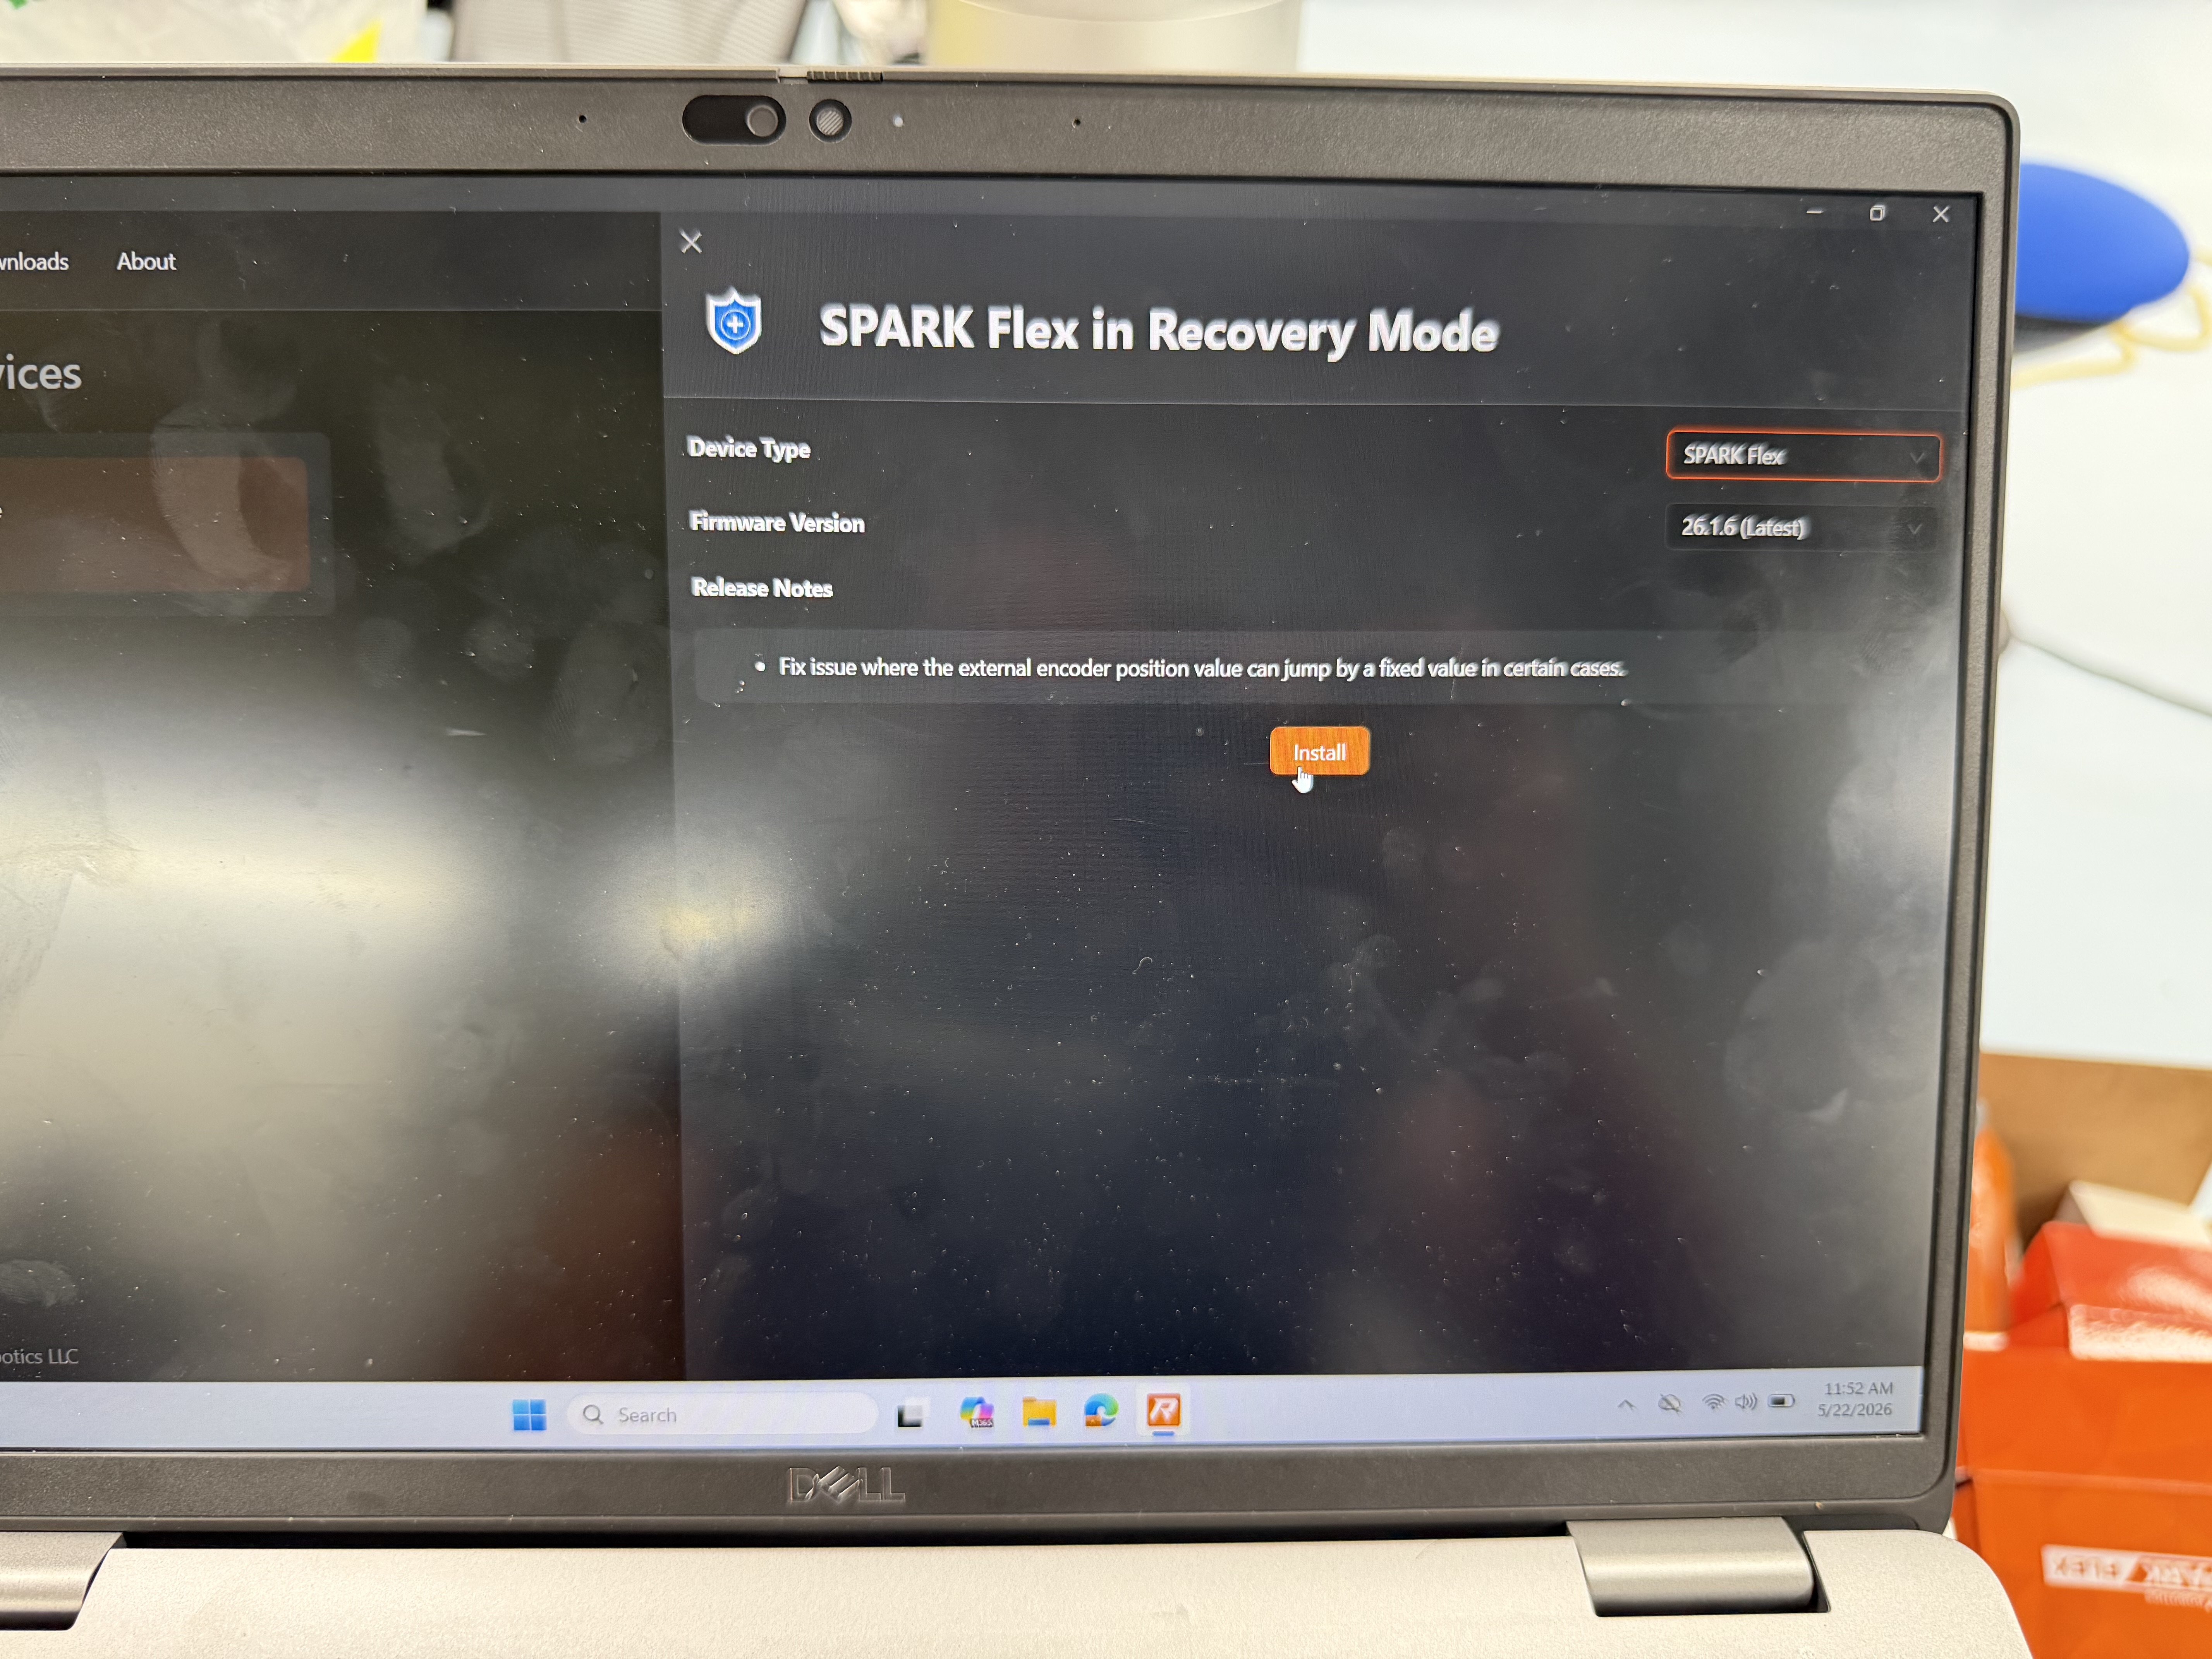
\includegraphics[width=0.5\textwidth]{media/image29.jpg}
\caption{Selecting SPARK Flex and the latest firmware on the recovery
device.}
\end{figure}
\clearpage

\assemblystep{Set the CAN ID}
Now you can change the CAN ID. It is recommended to start at a number
then increment with each motor as to avoid having the same ID. It is
also recommended to label the motor with the CAN ID to avoid confusion
later. The numbers used must match the IDs used in arm\_base\_control/configs/basename\_config.yaml file. Either use those values or update the file.

\begin{warningbox}
Make sure only one motor is plugged into the computer at a time while
setting up. As best practice, unplug the motor after the firmware is
successfully updated and then plug back in.
\end{warningbox}

\assemblystep{Configure Motor Settings}
Update the following configurations. Remember to click
the orange save button on the bottom right.



\rowcolors{2}{gray!10}{white}

\begin{table}[H]
\centering
\renewcommand{\arraystretch}{1.35}
\begin{tabularx}{\textwidth}{l X l}
\toprule
\rowcolor{sbotblue!15}
\textbf{Tab} & \textbf{Setting} & \textbf{Value} \\
\midrule
Basic & Idle Mode & \textbf{BRAKE} \\
Closed Loop Control & Closed Loop Control Sensor & \texttt{MAIN\_ENCODER} \\
Closed Loop Control Slot 0 & P0 & \texttt{Steer Motor: 0.5, Drive Motor: .119} \\
\bottomrule
\end{tabularx}
\caption{Required motor controller configuration settings.}
\end{table}

A complete list of configuration settings can be found in Appendix A.






